\FloatBarrier
\section{Results}\label{sec:results}

\begin{table*}[!htbp]\centering\small
\caption{Full-sample out-of-sample results, net of 10\,bps costs. CAGR, Vol, MaxDD, CVaR and TE$_{\text{HRP}}$ in \%; turnover annualised; Viol = share of rebalances breaching any constraint; $p$ = bootstrap $p$-value of the Sharpe difference with CA-HRP. Unconstrained methods (top block) are shown for reference only. Best constrained Sharpe ratio in bold.}\label{tab:main}
\setlength{\tabcolsep}{4.5pt}\begin{tabular}{llrrrrrrrrrr}\toprule
Universe & Method & CAGR & Vol & Sharpe & $p$ & MaxDD & CVaR$_{5}$ & Turn. & Viol & TE$_{\text{HRP}}$ & Eff.\,N\\\midrule
\multirow{11}{*}{\rotatebox{90}{Multi-asset ETFs}} & EW & 8.0 & 10.9 & 0.763 & 0.12 & -24.8 & -1.63 & 0.34 & 0\% & 10.2 & 20.0\\
 & IVP & 1.9 & 2.2 & 0.840 & 0.70 & -9.6 & -0.34 & 0.30 & 100\% & 0.5 & 1.6\\
 & MinVar & 2.4 & 2.4 & 0.971 & 0.68 & -9.1 & -0.36 & 0.90 & 100\% & 1.4 & 2.5\\
 & ERC & 4.8 & 5.7 & 0.852 & 0.47 & -17.3 & -0.84 & 0.48 & 100\% & 4.5 & 9.3\\
 & HRP & 1.6 & 2.0 & 0.833 & 0.70 & -8.8 & -0.30 & 0.63 & 100\% & 0.0 & 1.4\\
\cmidrule{2-12}
 & MinVar-C & 6.8 & 7.3 & \textbf{0.935} & 0.34 & -17.5 & -1.07 & 1.21 & 0\% & 6.5 & 8.0\\
 & MVO-C & 8.8 & 12.2 & 0.753 & 0.30 & -19.1 & -1.91 & 3.16 & 0\% & 11.6 & 7.3\\
 & HRP-Clip & 6.3 & 9.2 & 0.709 & 0.01 & -22.8 & -1.37 & 2.17 & 46\% & 8.4 & 13.9\\
 & HRP-Proj & 7.4 & 9.9 & 0.764 & 0.13 & -22.8 & -1.49 & 0.62 & 0\% & 9.3 & 16.1\\
 & CA-HRP-B & 7.1 & 9.8 & 0.750 & 0.14 & -21.4 & -1.47 & 2.50 & 0\% & 9.2 & 10.7\\
 & \textbf{CA-HRP} & 6.6 & 7.4 & 0.908 & -- & -18.8 & -1.08 & 1.25 & 0\% & 6.4 & 8.3\\
\midrule
\multirow{11}{*}{\rotatebox{90}{NIFTY 50 stocks}} & EW & 19.7 & 15.4 & 1.247 & 0.07 & -36.0 & -2.21 & 0.62 & 0\% & 3.7 & 43.0\\
 & IVP & 18.7 & 14.3 & 1.272 & 0.02 & -33.4 & -2.04 & 0.85 & 17\% & 2.0 & 37.8\\
 & MinVar & 18.0 & 12.8 & 1.356 & 0.89 & -26.1 & -1.74 & 2.87 & 100\% & 4.7 & 14.1\\
 & ERC & 19.5 & 14.2 & 1.326 & 0.22 & -32.7 & -2.02 & 0.81 & 3\% & 1.8 & 39.0\\
 & HRP & 19.5 & 13.7 & 1.368 & 0.96 & -30.6 & -1.94 & 2.70 & 48\% & 0.0 & 32.4\\
\cmidrule{2-12}
 & MinVar-C & 18.6 & 12.8 & \textbf{1.401} & 0.62 & -26.5 & -1.76 & 2.12 & 0\% & 3.5 & 19.8\\
 & MVO-C & 20.2 & 16.2 & 1.216 & 0.17 & -33.2 & -2.35 & 3.35 & 0\% & 6.8 & 17.4\\
 & HRP-Clip & 19.6 & 13.7 & 1.369 & 1.00 & -30.6 & -1.95 & 2.66 & 8\% & 0.2 & 32.8\\
 & HRP-Proj & 19.6 & 13.8 & 1.368 & 0.97 & -30.6 & -1.95 & 2.62 & 0\% & 0.2 & 32.9\\
 & CA-HRP-B & 19.5 & 13.7 & 1.368 & 0.68 & -30.1 & -1.95 & 2.51 & 0\% & 0.9 & 33.1\\
 & \textbf{CA-HRP} & 19.5 & 13.7 & 1.369 & -- & -30.1 & -1.94 & 2.47 & 0\% & 0.9 & 33.1\\
\midrule
\multirow{11}{*}{\rotatebox{90}{US large caps}} & EW & 13.3 & 18.5 & 0.767 & 0.59 & -47.9 & -2.80 & 0.53 & 0\% & 4.8 & 47.0\\
 & IVP & 11.7 & 16.1 & 0.768 & 0.15 & -41.1 & -2.40 & 0.73 & 24\% & 1.3 & 37.0\\
 & MinVar & 9.3 & 13.7 & 0.720 & 0.39 & -33.0 & -1.98 & 3.02 & 100\% & 6.2 & 10.5\\
 & ERC & 12.4 & 16.8 & 0.781 & 0.67 & -44.7 & -2.54 & 0.68 & 3\% & 2.3 & 42.6\\
 & HRP & 11.6 & 15.7 & 0.776 & 0.14 & -40.7 & -2.35 & 2.88 & 66\% & 0.0 & 33.9\\
\cmidrule{2-12}
 & MinVar-C & 10.7 & 14.5 & 0.773 & 0.66 & -35.7 & -2.15 & 2.06 & 0\% & 3.6 & 19.5\\
 & MVO-C & 12.7 & 17.5 & 0.774 & 0.82 & -43.2 & -2.64 & 3.43 & 0\% & 6.9 & 17.5\\
 & HRP-Clip & 11.6 & 15.8 & 0.775 & 0.12 & -41.1 & -2.37 & 2.80 & 8\% & 0.3 & 34.6\\
 & HRP-Proj & 11.7 & 15.8 & 0.775 & 0.11 & -41.2 & -2.37 & 2.76 & 0\% & 0.3 & 34.7\\
 & CA-HRP-B & 11.9 & 15.8 & 0.790 & 0.55 & -41.9 & -2.36 & 2.65 & 0\% & 1.0 & 34.8\\
 & \textbf{CA-HRP} & 11.9 & 15.7 & \textbf{0.793} & -- & -40.4 & -2.35 & 2.57 & 0\% & 0.9 & 34.7\\
\bottomrule
\end{tabular}\end{table*}

\subsection{Constraint compliance}
Table~\ref{tab:main} first answers the practical question. Unconstrained HRP breaches the
mandate at 100\% of rebalances in the multi-asset universe, 48\% for NIFTY and 66\% for
US stocks. The common practitioner fix, HRP-Clip, still breaches constraints at 46\%, 8\%
and 8\% of rebalances respectively: alternating clipping and group rescaling can cycle
when per-asset and group limits interact, and it ignores turnover entirely. Every
optimisation-based method, including both CA-HRP variants, satisfies all constraints at
every rebalance, and CA-HRP never needed the turnover fallback.

\subsection{Performance where constraints bind}
The multi-asset universe is where constraints bite hardest: HRP would hold on average 86\%
in a single short-term Treasury fund (Figure~\ref{fig:groups}), so the 15\% fund cap, the
40\% asset-class cap and the 20\% equity floor force a very different portfolio. Here the
way the constraints are enforced matters a great deal. CA-HRP reaches a Sharpe ratio of
0.908 with 7.4\% volatility and a $-18.8\%$ maximum drawdown, against 0.764, 9.9\% and
$-22.8\%$ for the Euclidean projection (HRP-Proj) and 0.709 for HRP-Clip. The difference with
HRP-Clip is significant ($p=0.01$); against HRP-Proj and equal weight the $p$-values are
0.13 and 0.12. Among all constrained methods, only constrained minimum variance has a higher
Sharpe ratio (0.935), a difference that is far from significant ($p=0.34$). CA-HRP's
realised tracking error to HRP (6.4\%) is the lowest of the HRP-family methods, as its
construction intends.

The solver-free CA-HRP-B performs like the Euclidean projection (0.750) but with four
times the turnover. Its bisection handles constraints by pushing excess weight down the
tree, so the portfolio concentrates in whichever volatile branch has spare capacity
(commodities, Figure~\ref{fig:groups} and Section~\ref{sec:method}). This is the central
negative finding that motivated the final design: constraints are best enforced
\emph{after} the risk allocation, in a risk metric, not inside the bisection.

\begin{figure}[t]
\centering
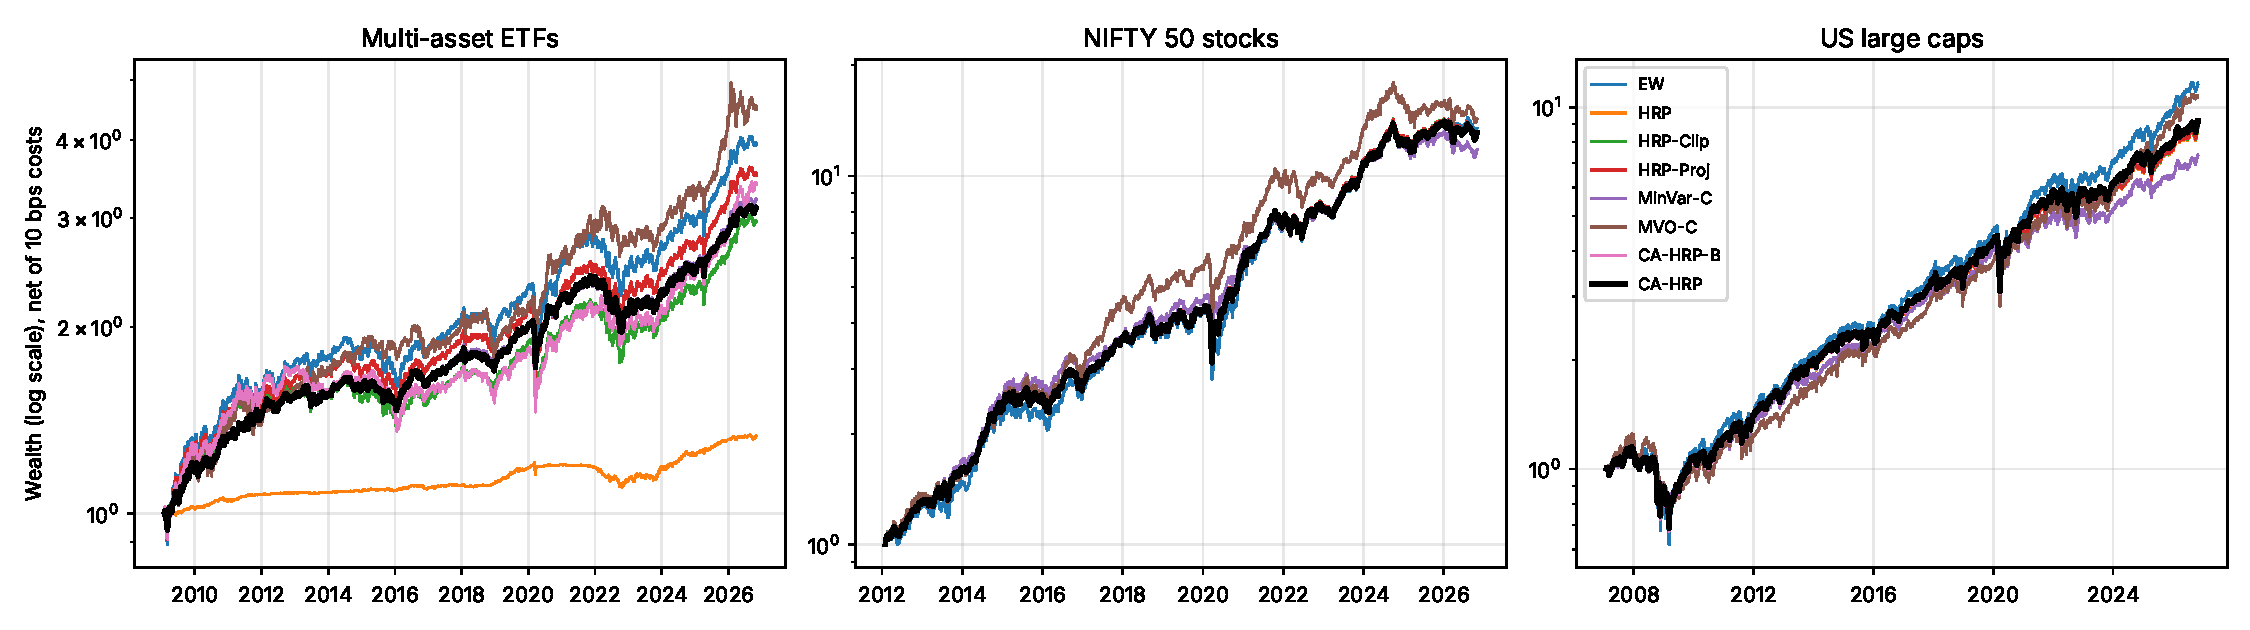
\includegraphics[width=\linewidth]{../results/figures/wealth_curves.pdf}
\caption{Growth of one unit of wealth (log scale), net of 10\,bps costs.}
\label{fig:wealth}
\end{figure}

\begin{figure}[t]
\centering
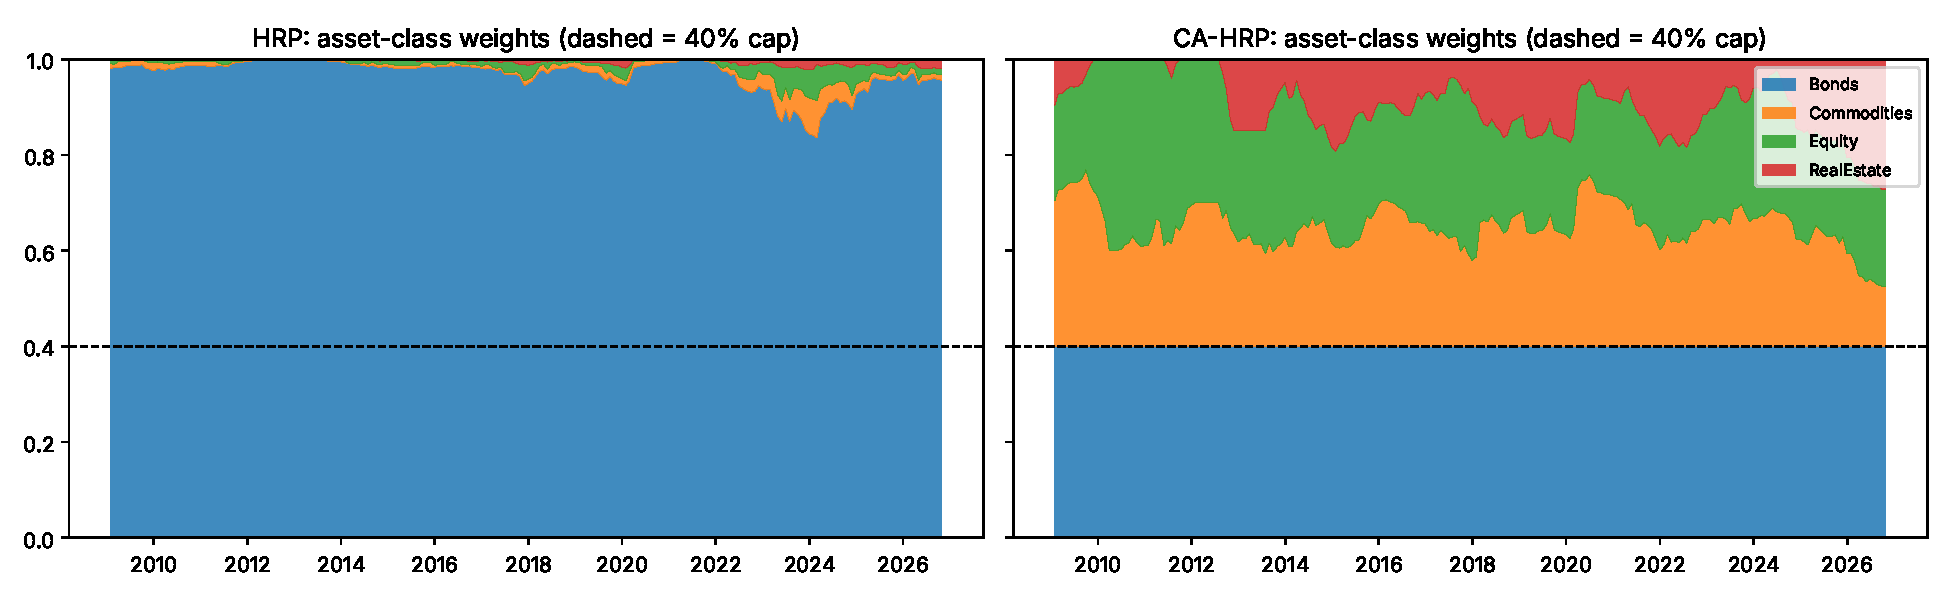
\includegraphics[width=\linewidth]{../results/figures/etf_group_weights.pdf}
\caption{Asset-class weights in the multi-asset universe. Unconstrained HRP (left) is
almost entirely in bonds, far above the 40\% cap. CA-HRP (right) holds bonds at the cap
and allocates the remainder by tracking-error projection.}
\label{fig:groups}
\end{figure}

\subsection{Performance where constraints rarely bind}
In the two stock universes HRP breaches the limits at about half of the rebalances, but only
by small amounts: the realised tracking error between HRP and any of its constrained
versions is at most 1\%. All HRP-based methods are therefore statistically indistinguishable,
which is what Proposition~\ref{prop:te}(b) predicts as the constraints become slack. CA-HRP posts the highest Sharpe ratio
of all eleven methods for US large caps (0.793) and ties HRP for NIFTY (1.369 vs 1.368),
where constrained minimum variance is marginally higher (1.401, $p=0.62$). In other words,
CA-HRP costs nothing when HRP is already compliant and helps when it is not.

\subsection{Held-out test period}
Table~\ref{tab:test} repeats the comparison on the period after the validation window,
which played no role in choosing the design. The ranking is unchanged. In the multi-asset
universe CA-HRP's test Sharpe is 0.929, against 0.805 for HRP-Proj, 0.802 for HRP-Clip,
0.783 for equal weight and 0.977 for constrained minimum variance, with the lowest
volatility of any HRP-family method. In stocks CA-HRP again matches HRP.

\begin{table}[!htbp]\centering\small
\caption{Sharpe ratio (net of 10\,bps) on the held-out test period, which was never used to choose the CA-HRP design, next to the full sample. Vol and MaxDD (\%) on the test period.}\label{tab:test}
\begin{tabular}{l rrr rrr}\toprule
 & \multicolumn{3}{c}{Test-period Sharpe} & \multicolumn{3}{c}{ETFs, test period}\\
\cmidrule(lr){2-4}\cmidrule(lr){5-7}
Method & ETFs & NIFTY & US & Vol & MaxDD & Full-sample SR\\\midrule
EW & 0.783 & 1.066 & 0.972 & 10.6 & -24.8 & 0.763\\
HRP & 0.830 & 1.126 & 0.909 & 2.4 & -8.8 & 0.833\\
MinVar-C & 0.977 & 1.051 & 0.889 & 7.4 & -17.5 & 0.935\\
MVO-C & 0.781 & 0.869 & 0.976 & 12.9 & -19.1 & 0.753\\
HRP-Clip & 0.802 & 1.126 & 0.909 & 8.9 & -22.8 & 0.709\\
HRP-Proj & 0.805 & 1.126 & 0.910 & 9.6 & -22.8 & 0.764\\
CA-HRP-B & 0.876 & 1.122 & 0.947 & 9.5 & -21.3 & 0.750\\
\textbf{CA-HRP} & 0.929 & 1.123 & 0.941 & 7.4 & -18.8 & 0.908\\
\bottomrule\end{tabular}\end{table}

\subsection{Ablation}
Table~\ref{tab:ablation} isolates each design choice. In the multi-asset universe the
\emph{distance metric} drives almost the whole gain: replacing the full-covariance
tracking-error metric by its diagonal lowers the Sharpe ratio from 0.908 to 0.777, and the
Euclidean metric to 0.742. Adding capacity-aware bisection before the projection lowers it
to 0.861 and nearly doubles turnover; adding a tree-consistency penalty has a similar
effect. The choice of covariance estimator, linkage rule and split rule matters little
(Sharpe 0.910--0.922), so the method is not sensitive to those HRP details. Removing the
turnover cap barely changes performance, showing that the cap is rarely binding for CA-HRP
and does not drive its results. In the stock universes no ablation moves the Sharpe ratio
by more than 0.04.

\begin{table}[!htbp]\centering\small
\caption{Ablation of CA-HRP components (full sample, net of 10\,bps). Each row changes one component of the full method.}\label{tab:ablation}
\begin{tabular}{l rrr rrr}\toprule
 & \multicolumn{3}{c}{Sharpe ratio} & \multicolumn{3}{c}{ETFs}\\
\cmidrule(lr){2-4}\cmidrule(lr){5-7}
Variant & ETFs & NIFTY & US & Vol & Turn. & TE$_{\text{HRP}}$\\\midrule
CA-HRP (full) & 0.908 & 1.369 & 0.793 & 7.4 & 1.25 & 6.4\\
\midrule
sample covariance & 0.922 & 1.372 & 0.781 & 7.3 & 1.22 & 6.4\\
diagonal metric & 0.777 & 1.366 & 0.791 & 9.2 & 1.14 & 8.5\\
Euclidean metric & 0.742 & 1.365 & 0.789 & 9.8 & 1.06 & 9.1\\
+ capacity bisection & 0.861 & 1.367 & 0.796 & 8.5 & 2.30 & 7.7\\
+ tree-consistency term & 0.846 & 1.370 & 0.794 & 7.9 & 2.27 & 7.1\\
no turnover cap & 0.910 & 1.369 & 0.793 & 7.3 & 1.26 & 6.4\\
Ward linkage & 0.910 & 1.330 & 0.759 & 7.4 & 1.30 & 6.4\\
dendrogram splits & 0.918 & 1.392 & 0.778 & 7.4 & 1.19 & 6.5\\
\bottomrule\end{tabular}\end{table}

\subsection{Robustness}
\paragraph{Costs and estimation window.} Table~\ref{tab:robust} shows the multi-asset
advantage of CA-HRP over the other HRP-family methods survives 50\,bps costs (0.840 vs 0.739
for HRP-Proj) and both shorter (126-day) and longer (504-day) estimation windows, where
CA-HRP improves on HRP-Proj by 0.14 and 0.19 Sharpe points respectively. Constrained minimum
variance remains a strong competitor throughout.

\paragraph{Stability of weights.} We re-estimate every method on 30 block-bootstrapped
versions of the estimation window at eight dates per universe and measure how much the
weights move. CA-HRP is far more stable than mean--variance (instability 0.16--0.22 vs
0.70--0.78) and more stable than constrained minimum variance in every universe (e.g.\
0.218 vs 0.324 for NIFTY). In the multi-asset universe HRP-Proj is the most stable, because
it is anchored near equal weight; its stability comes at the price of a portfolio that
tracks HRP poorly and has higher volatility.

\begin{table*}[!htbp]\centering\small
\caption{Robustness. Left: Sharpe ratio in the multi-asset universe at 50\,bps costs and with 126- and 504-day estimation windows (all universes). Right: weight instability, the mean $L_1$ distance of bootstrapped weights from their average (lower = more stable).}\label{tab:robust}
\begin{tabular}{l r rrr rrr rrr}\toprule
 & ETFs & \multicolumn{3}{c}{Window 126 days} & \multicolumn{3}{c}{Window 504 days} & \multicolumn{3}{c}{Weight instability}\\
\cmidrule(lr){3-5}\cmidrule(lr){6-8}\cmidrule(lr){9-11}
Method & 50\,bps & ETFs & NIFTY & US & ETFs & NIFTY & US & ETFs & NIFTY & US\\\midrule
EW & 0.750 & 0.535 & 1.197 & 0.794 & 0.701 & 1.196 & 0.775 & -- & -- & --\\
HRP & 0.705 & 0.622 & 1.288 & 0.786 & 0.932 & 1.287 & 0.767 & 0.068 & 0.230 & 0.227\\
MinVar-C & 0.868 & 0.703 & 1.392 & 0.801 & 0.936 & 1.341 & 0.730 & 0.185 & 0.324 & 0.318\\
MVO-C & 0.650 & 0.660 & 1.142 & 0.755 & 0.796 & 1.172 & 0.760 & 0.754 & 0.698 & 0.781\\
HRP-Clip & 0.614 & 0.479 & 1.293 & 0.786 & 0.800 & 1.288 & 0.767 & 0.209 & 0.222 & 0.214\\
HRP-Proj & 0.739 & 0.535 & 1.293 & 0.792 & 0.714 & 1.288 & 0.766 & 0.037 & 0.220 & 0.217\\
\textbf{CA-HRP} & 0.840 & 0.676 & 1.301 & 0.803 & 0.908 & 1.276 & 0.766 & 0.158 & 0.218 & 0.211\\
\bottomrule\end{tabular}\end{table*}

\paragraph{Stress periods.} Table~\ref{tab:stress} reports cumulative returns in three
crises. In the COVID crash CA-HRP lost 6.9\% in the multi-asset universe, against 14.0\% for
HRP-Proj, 13.7\% for HRP-Clip and 14.9\% for equal weight, and it was flat in the GFC window.
The 2022 rates shock is the exception: CA-HRP's hedge tilt towards intermediate and long
Treasuries, which protected it in 2020, lost 17.2\% when bonds and equities fell together,
slightly more than HRP-Proj ($-15.3\%$). This illustrates the main limitation of any
covariance-based hedge: it relies on correlations that can break down.

\begin{table}[!htbp]\centering\small
\caption{Cumulative return (\%) in stress windows: GFC = Sep 2008--Mar 2009, COVID = 15 Feb--30 Apr 2020, Rates = Jan--Oct 2022.}\label{tab:stress}
\setlength{\tabcolsep}{4pt}\begin{tabular}{l rrr r rrr}\toprule
 & \multicolumn{3}{c}{ETFs} & NIFTY & \multicolumn{3}{c}{US}\\
\cmidrule(lr){2-4}\cmidrule(lr){5-5}\cmidrule(lr){6-8}
Method & GFC & COVID & Rates & COVID & GFC & COVID & Rates\\\midrule
EW & -1.6 & -14.9 & -16.9 & -16.8 & -30.4 & -13.5 & -5.1\\
HRP & 0.6 & -0.3 & -6.6 & -9.6 & -24.8 & -10.0 & -5.9\\
MinVar-C & 0.5 & -7.6 & -16.0 & -4.4 & -20.3 & -10.7 & -4.4\\
MVO-C & 0.8 & -4.5 & -8.2 & -13.8 & -30.1 & -9.3 & -0.9\\
HRP-Clip & 0.4 & -13.7 & -17.4 & -9.6 & -24.8 & -10.0 & -6.3\\
HRP-Proj & -1.0 & -14.0 & -15.3 & -9.6 & -25.0 & -10.0 & -6.3\\
CA-HRP-B & -2.2 & -11.2 & -11.3 & -8.4 & -25.8 & -9.0 & -5.3\\
\textbf{CA-HRP} & 0.3 & -6.9 & -17.2 & -8.4 & -24.7 & -9.5 & -5.4\\
\bottomrule\end{tabular}\end{table}

\paragraph{Tightening the constraints.} Finally, we tighten the per-asset cap from $4/N$ to
$1.25/N$ (with group caps scaled accordingly) and measure, at twelve dates per universe, how
far each method's portfolio is from HRP in ex-ante tracking-error terms
(Figure~\ref{fig:tight}). Settings that are mathematically infeasible (caps of $1.5/N$ and
$1.25/N$ in the multi-asset universe) are detected by a linear feasibility check and
skipped; HRP-Clip silently returns infeasible weights in such cases, and even at caps of
$2.5/N$ and looser it still breaches limits by 1.1--1.9 percentage points on average in the
multi-asset universe. In that universe CA-HRP has the smallest distortion at every cap
(7.1--9.2\% versus 10.5--11.9\% for HRP-Proj) and the lowest volatility. In the stock
universes CA-HRP has a small constant floor of about 0.8\% because its HRP target uses
shrinkage rather than the sample covariance; at the tightest cap ($1.25/N$) it distorts HRP
the least in both stock universes (2.2\% vs 2.4--2.5\% for NIFTY, 2.8\% vs 3.2--3.3\% for US),
and already at $1.5/N$ for US stocks.

\begin{figure}[t]
\centering
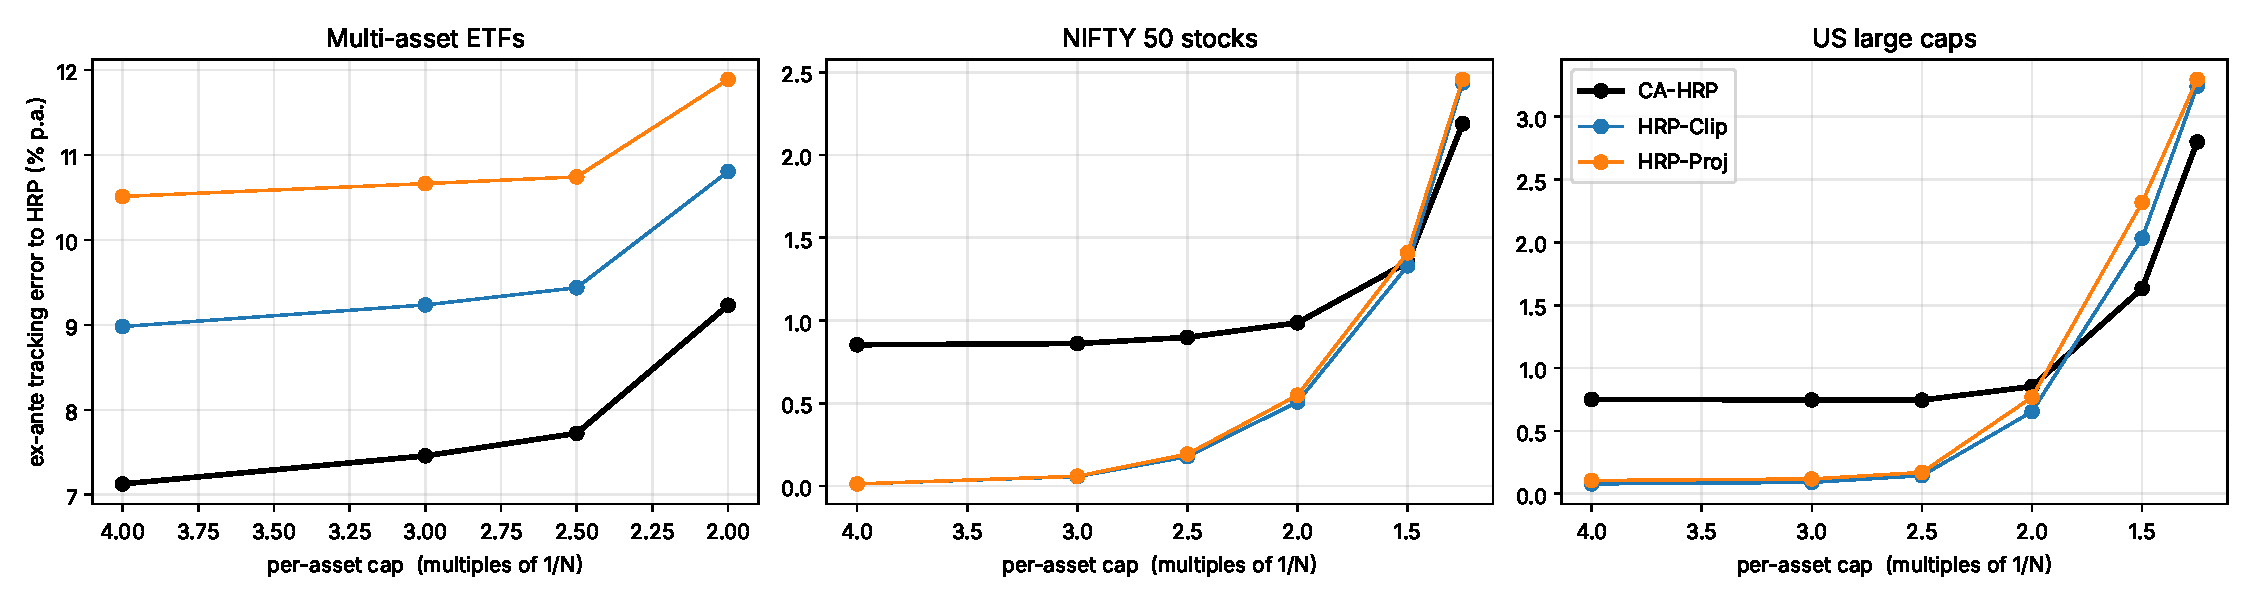
\includegraphics[width=\linewidth]{../results/figures/tightness.pdf}
\caption{Ex-ante tracking error to sample-covariance HRP as the per-asset cap tightens
(right = tighter). Infeasible settings are omitted.}
\label{fig:tight}
\end{figure}

\FloatBarrier
\section{Discussion}\label{sec:discussion}
Three lessons emerge. First, \emph{HRP is not deployable as-is} under realistic mandates:
it breaches constraints at up to every rebalance, and the clipping fix used in practice still
fails often. Second, \emph{how} constraints are enforced matters as much as \emph{whether}
they are: the same HRP target, projected with a risk-aware metric instead of a Euclidean one,
gives a portfolio with 25\% less volatility and a higher Sharpe ratio, out of sample and in
the held-out period. Third, building constraints into the bisection, while elegant and
provably feasible, is inferior to separating risk allocation from constraint enforcement.

\paragraph{Limitations.} The stock universes are survivorship-biased because they contain
current large caps; this affects all methods equally. The gains of CA-HRP are concentrated
in settings where constraints bind strongly; when they do not, it reduces to HRP, which is
by design. Most Sharpe differences are not statistically significant at conventional
levels, which is typical for portfolio comparisons over 15--20 years, and constrained
minimum variance remains a strong benchmark. Finally, the tracking-error projection
inherits the weakness of any covariance-based hedge, visible in 2022 when stock--bond
correlation turned positive.
